\section{Wprowadzenie do tematyki}



\subsection{Terminologia użyta w~pracy}
Zgodnie z~terminologią stosowaną w~kryptologii, w~pracy konsekwentnie
wykorzystywane będą następujące pojęcia:

\begin{itemize}

    \item \textbf{funkcja haszująca}~-- alternatywne określenie \emph{funkcji
    skrótu},

    \item \textbf{bezpieczna funkcja haszująca}~-- alternatywne określenie
    \emph{kryptograficznej funkcji skrótu},

    \item \textbf{zwykła funkcja haszująca}~-- funkcja skrótu, która może, ale
    nie musi być \emph{kryptograficzną funkcją skrótu},

    \item \textbf{wiadomość}~-- wartość wejściowa dla \emph{funkcji skrótu},

    \item \textbf{skrót}~-- wartość wyjściowa z~\emph{funkcji skrótu},

    \item \textbf{hasz}~-- alternatywne określenie na wartość wyjściową
    \emph{funkcji skrótu},

    \item \textbf{kolizja}~-- sytuacja, w~której skróty dwóch różnych
    wiadomości są takie same, tj.
    \[
        \begin{aligned}
        m &\neq m' \\
        H(m) &= H(m')
        \end{aligned}
    \]

    \item \textbf{zadanie praktycznie niewykonalne}~-- algorytm, który
    realizuje dane zadanie, nie istnieje, albo jego koszt obliczeniowy lub
    pamięciowy jest tak wielki, że nie można go wykonać przy pomocy znanych
    obecnie technologii.

\end{itemize}

Dodatkowo, od części~\ref{sec:hash_construction} do końca pracy przez pojęcie
funkcji haszujących będziemy rozumieć wyłącznie kryptograficzne funkcje
haszujące, gdyż tylko na takich funkcjach w~tych częściach będziemy się
skupiać.
\pagebreak



\subsection{Definicja zwykłej oraz kryptograficznej funkcji skrótu}
Funkcja skrótu jest to funkcja, której dziedziną są ciągi bitów dowolnej
długości, a~przeciwdziedziną~-- ciągi bitów o~stałej, ograniczonej długości.
Rzutowanie to odbywa się w~sposób jednoznaczny, tj. każdemu wejściu funkcja
skrótu przyporządkowuje dokładnie jedno wyjście; formalnie zatem jest to
surjekcja:

$$ f \colon X \to Y $$
$$ |Y| \leq n, n \in \mathbb{N} $$
$$ \forall_{y \in Y} \; \exists_{x \in X} \; f(x)=y $$

\begin{figure}[htb!]
    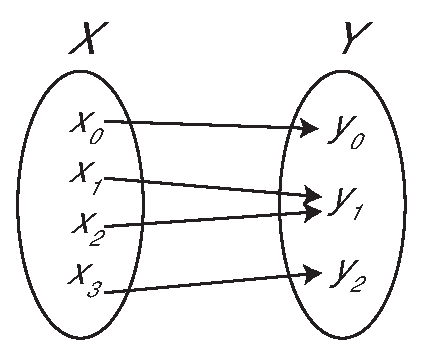
\includegraphics[width=6cm]{img/surjection.eps}
    \caption{Każdemu wejściu przyporządkowywane jest dokładnie jedno wyjście}
    \label{fig:surjection}
\end{figure}

Kryptograficzna funkcja skrótu to taka funkcja skrótu, która może być
wykorzystywana w~zastosowaniach kryptograficznych, a~więc wymagających
wysokiego poziomu bezpieczeństwa. Przykłady takich zastosowań można znaleźć
w~sekcji~\ref{sec:secure_hash_usages}. Dokładne cechy, jakie powinna spełniać
funkcja skrótu, aby była kryptograficzna, omówione zostały w~sekcji
~\ref{sec:secure_hash_attributes}. Ponadto wszystkie funkcje skrótu,
niezależnie od swojego zastosowania w~celach kryptograficznych, powinny
spełniać własności opisane w~sekcji~\ref{sec:common_hash_attributes}.



\subsubsection{Cechy zwykłych funkcji haszujących}
\label{sec:common_hash_attributes}
Niezależnie od swojego zastosowania, każda funkcja haszująca musi spełniać
pewne warunki, które zostały poniżej opisane.

\myparagraph{Determinizm}
Funkcje haszujące powinny być deterministyczne w~takim sensie, że ich wyniki
zależą wyłącznie od danych wejściowych, a~nie żadnych czynników losowych.
Innymi słowy, haszowanie wiadomości $m$ powinno dawać taki sam skrót
niezależnie od okoliczności. Stąd wynika, że funkcje skrótu nie powinny się
nigdy odwoływać do generatorów liczb pseudolosowych, metadanych o~wiadomości
(typu jej lokalizacja w~pamięci komputera) itp., a~jedynie do samej wiadomości.

\myparagraph{Jednostajność}
Niech $H : A \to B$ będzie funkcją haszującą. Funkcje haszujące powinny
przekształcać wartości ze zbioru wejściowego $A$ na wartości ze zbioru
wyjściowego $B$ w~taki sposób, by:
\[
    \forall_{a \in A} \; \Pr(H(a) = b) \to \frac{1}{|B|}
\]
Innymi słowy dobra funkcja haszująca przekształca konkretną wartość $a$
w~konkretną wartość $b$ z~prawdopodobieństwem jak najbliższym
prawdopodobieństwu losowego wybrania tego elementu ze zbioru $B$, lub też~--
dla danej wiadomości $m$ wszystkie wartości ze zbioru $B$ powinny mieć możliwie
taką samą szansę na wybranie (z zachowaniem własności determinizmu). Cecha ta
ma na celu zapewnienie jak najmniejszego prawdopodobieństwa zajścia kolizji.

Unikanie kolizji, obok determinizmu, jest jedną z~najważniejszych cech funkcji
skrótu, co staje się zrozumiałe, gdy pozna się ich zastosowania (przykładowe
zastosowania bezpiecznych funkcji skrótu opisane są
w~sekcji~\ref{sec:secure_hash_usages}).



\subsubsection{Cechy kryptograficznych funkcji haszujących}
\label{sec:secure_hash_attributes}
Aby lepiej zrozumieć naturę warunków nałożonych na cechy kryptograficznych, lub
też \emph{bezpiecznych} funkcji skrótu, należy uświadomić sobie ich naturę:
w~sytuacji, kiedy kolizje są tylko niepożądane, sięgamy po zwykłe funkcje
haszujące, funkcje kryptograficzne stają się natomiast potrzebne wówczas, gdy
kolizje są \emph{niedopuszczalne}.

Jednak z~racji mniejszego rozmiaru przeciwdziedziny w~stosunku do dziedziny
(patrz rysunek~\ref{fig:surjection} na stronie \pageref{fig:surjection}),
kolizje \emph{będą} się zdarzać.

Poniższe warunki zostały sformułowane po to, aby sytuacje, w~których dochodzi
do kolizji, były jak najmniej prawdopodobne i~żeby było trudno je celowo
wywołać, a~także żeby same kryptograficzne funkcje skrótu stanowiły godne
użycia narzędzie we wszystkich sytuacjach, które wymagają wysokiego
bezpieczeństwa.

\myparagraph{Odporność na kolizje pierwszego rzędu (\en{preimage resistance})}
\label{sec:preimage_resistance}
Mając dany skrót $h$, znalezienie wiadomości $m$ takiej, że $H(m) = h$ powinno
być w~praktyce niewykonalne. Jest to warunek zapewniający jednostronność
funkcji skrótu. Należy zauważyć, że zależy nam na \emph{dowolnej} wiadomości,
a~nie oryginalnej wiadomości z~której zostało utworzone $h$.

\myparagraph{Odporność na kolizje drugiego rzędu (\en{second preimage
resistance})}
\label{sec:second_preimage_resistance}
Mając daną wiadomość $m$, znalezienie wiadomości $m' \neq m$ takiej, że $H(m) =
H(m')$ powinno być praktycznie niewykonalne.

\myparagraph{Odporność na kolizje (\en{collision resistance})}
\label{sec:collision_resistance}
Znalezienie dwóch dowolnych różnych wiadomości $m \neq m'$ takich, że $H(m) =
H(m')$ powinno być praktycznie niewykonalne. Spełnienie tej własności implikuje
odporność na kolizje drugiego rzędu, co jednak nie implikuje odporności na
kolizje pierwszego rzędu.

\myparagraph{Niemożność odróżnienia od \en{random oracles}}
\en{Random oracle} to teoretyczna czarna skrzynka przypisująca każdemu
argumentowi losową (z jednostajnym rozkładem prawdopodobieństwa) wartość
z~określonej przeciwdziedziny w~taki sposób, że dla konkretnego argumentu
zawsze wybiera taką samą wartość. Jest to abstrakcyjna funkcja matematyczna,
o~której udowodniono~\cite{random_oracle}, że nie może posiadać żadnej
implementacji.\renmich{Oj, to chyba niezupełnie tak. Chciałbym o~tym porozmawiać.} Pożądane jest to, by kryptograficzna funkcja skrótu była trudna
do odróżnienia od \en{random oracle}, choć jest to zadanie znacznie trudniejsze
od spełnienia poprzednich własności.

\myparagraph{Własność efektu lawinowego}
\label{sec:avalance_effect}
W~dobrych funkcjach haszujących powinien zachodzić tzw. efekt lawinowy. Jest to
własność zapewniająca, że nawet mała zmiana wiadomości $m'$ w~stosunku do $m$
powoduje duże zmiany w~wartości $H(m')$ w~porównaniu do $H(m)$. Jej celem jest
zapewnienie drugiej z~dwóch fundamentalnych własności dobrego systemu
kryptograficznego, sformułowanych przez Shannona
w~1949~\cite{confusion_diffusion}:

\begin{itemize}

    \item \en{confusion} (zamieszanie) -- zależność między szyfrogramem
    a~kluczem symetrycznym powinna być jak najbardziej skomplikowana
    i~nieprzewidywalna,

    \item \en{diffusion} (rozpraszanie) -- zależność między szyfrogramem
    a~tekstem jawnym powinna być jak najbardziej skomplikowana
    i~nieprzewidywalna.

\end{itemize}

Spełnienie tych warunków utrudnia potencjalne ataki.

\noindent Mówi się o~dwóch, wymienionych poniżej, kryteriach efektu
lawinowego~\cite{avalanche_criterion1,avalanche_criterion2}.

\begin{myenumerate}

    \item Ścisłe kryterium lawinowe (\en{strict avalanche criterion},
    \abbr{SAC}): po zmianie dowolnego bitu wejścia, każdy bit wyjścia powinien
    się zmienić z~prawdopodobieństwem równym $\frac{1}{2}$.

    Formalnie funkcja $f : \mathbb{Z}_2^n \to \mathbb{Z}_2^m$ spełnia ścisłe
    kryterium lawinowe, gdy:

    $$\forall i,j \; \sum_{x \in \mathbb{Z}_2^n} D_H(f(x) \oplus f(x \oplus
    C_i^n)) = m 2^{n-1}$$

    gdzie $D_H$ oznacza odległość Hamminga, a $C_i^n$ oznacza $i$-ty wiersz
    macierzy identyczności $I$ (czyli wektor złożonych z~1 na $i$-tym miejscu
    i~0 na pozostałych miejscach).

    \item Kryterium niezależności bitowej (\en{bit independence criterion},
    \abbr{BIC}): po zmianie dowolnego bitu wejścia, każde dwa bity wyjścia
    powinny zmieniać się w~sposób niezależny od siebie.

    Możliwe jest ocenienie stopnia, w~jakim dana funkcja $f$ spełnia kryterium
    niezależności bitowej. Formalnie:

    $$BIC(f) = \max_{x, y \in \mathbb{Z}_2^n} \left( \max_{1 \leq i \leq n}
    |corr(f(x) \oplus (f(x) \oplus C_i^n), f(y) \oplus (f(y) \oplus C_i^n))|
    \right)$$

    W~najlepszym wypadku $BIC(f) = 0$, w~najgorszym $BIC(f) = 1$.

\end{myenumerate}

\begin{figure}[hbt!]
    \pgfplotsset{width=14cm,height=7cm}
    \begin{tikzpicture}
        \newcommand{\tmp}{$\Pr(H(a)_{(2,i)}=1)$}
        \begin{axis}[xlabel=$i$-ty bit,ylabel=\tmp,/pgf/number
        format/.cd,fixed,precision=3]
        \addplot[color=blue,mark=*] coordinates {
            (0, 0.501249577499)
            (1, 0.50207665441)
            (2, 0.500985834708)
            (3, 0.500601743263)
            (4, 0.498658240554)
            (5, 0.499766984524)
            (6, 0.50055309168)
            (7, 0.498996241025)
            (8, 0.50000256061)
            (9, 0.500978152879)
            (10, 0.499813075497)
            (11, 0.500092181947)
            (12, 0.500104984995)
            (13, 0.500038409144)
            (14, 0.499416181004)
            (15, 0.500189485113)
            (16, 0.500914137638)
            (17, 0.499784908791)
            (18, 0.49979515123)
            (19, 0.499108907849)
            (20, 0.499188286747)
            (21, 0.501026804462)
            (22, 0.49944690832)
            (23, 0.501011440804)
            (24, 0.500547970461)
            (25, 0.49958262063)
            (26, 0.49972345416)
            (27, 0.500340561081)
            (28, 0.500975592269)
            (29, 0.498632634458)
            (30, 0.500924380076)
            (31, 0.500058894021)
            (32, 0.499833560374)
            (33, 0.500975592269)
            (34, 0.499229256501)
            (35, 0.500862925445)
            (36, 0.499746499647)
            (37, 0.500788667766)
            (38, 0.499434105272)
            (39, 0.500023045487)
            (40, 0.500842440568)
            (41, 0.498863089324)
            (42, 0.4979259062)
            (43, 0.500245818524)
            (44, 0.499352165764)
            (45, 0.500660637285)
            (46, 0.49937521125)
            (47, 0.499946227198)
            (48, 0.499559575144)
            (49, 0.500455788514)
            (50, 0.500325197423)
            (51, 0.499492999293)
            (52, 0.499490438684)
            (53, 0.499341923325)
            (54, 0.500399455102)
            (55, 0.50075794045)
            (56, 0.499221574672)
            (57, 0.500535167413)
            (58, 0.500862925445)
            (59, 0.499869408909)
            (60, 0.501812911618)
            (61, 0.501142031895)
            (62, 0.500194606332)
            (63, 0.501666956869)
            (64, 0.501326395788)
            (65, 0.499114029068)
            (66, 0.498932225784)
            (67, 0.49992830293)
            (68, 0.499149877603)
            (69, 0.499718332941)
            (70, 0.500181803284)
            (71, 0.49868384665)
            (72, 0.498258785452)
            (73, 0.501003758975)
            (74, 0.499784908791)
            (75, 0.499211332234)
            (76, 0.499664560138)
            (77, 0.501646471992)
            (78, 0.49889381664)
            (79, 0.500637591798)
            (80, 0.499536529657)
            (81, 0.499526287218)
            (82, 0.499500681122)
            (83, 0.5010370469)
            (84, 0.500299591327)
            (85, 0.4996543177)
            (86, 0.499969272684)
            (87, 0.498530210072)
            (88, 0.499974393904)
            (89, 0.499528847828)
            (90, 0.500094742556)
            (91, 0.500094742556)
            (92, 0.499769545133)
            (93, 0.500737455573)
            (94, 0.500875728493)
            (95, 0.500722091916)
            (96, 0.500542849242)
            (97, 0.499431544662)
            (98, 0.500778425328)
            (99, 0.499244620159)
            (100, 0.499989757561)
            (101, 0.498786271035)
            (102, 0.500578697776)
            (103, 0.500169000236)
            (104, 0.499841242203)
            (105, 0.50027398523)
            (106, 0.500156197187)
            (107, 0.500640152407)
            (108, 0.499116589678)
            (109, 0.500645273627)
            (110, 0.500099863776)
            (111, 0.49951348417)
            (112, 0.499918060492)
            (113, 0.500512121926)
            (114, 0.49979515123)
            (115, 0.499669681358)
            (116, 0.500225333647)
            (117, 0.501841078324)
            (118, 0.499879651347)
            (119, 0.498970634929)
            (120, 0.500312394375)
            (121, 0.50041481876)
            (122, 0.499160120041)
            (123, 0.499188286747)
            (124, 0.49889381664)
            (125, 0.500145954749)
            (126, 0.499733696598)
            (127, 0.500734894964)
        };
        \end{axis}
    \end{tikzpicture}
    \caption{Przykładowy rozkład prawdopodobieństwa występowania ``1'' na
    kolejnych bitach skrótów \texttt{MD5}, otrzymanych z~zahaszowania wyrazów
    z~listy~\ref{wl:english_wordlist} w~dodatku~\ref{app:wordlists}.}
    %todo: wspomnieć o programie z dodatku C
    \end{figure}
\pagebreak



\subsection{Zastosowania kryptograficznych funkcji skrótu}
\label{sec:secure_hash_usages}
Same funkcje skrótu mają bardzo szerokie zastosowania, my jednak skupimy się
wyłącznie na zastosowaniach \emph{kryptograficznych} funkcji haszujących.
W~każdym przypadku opisane zastosowanie utylizuje podstawową cechę
kryptograficznych funkcji skrótu, jaką jest odporność na kolizje.



\subsubsection{Weryfikacja integralności danych}
\label{sec:usage_integrity_check}
Wyobraźmy sobie sytuację, w~której użytkownik o~imieniu Alicja zmuszony jest
przetransportować jakieś dane przez niebezpieczny kanał informacji, który jest
podatny na zakłócenia, do użytkownika imieniem Bob. Niech wiadomość wysłana
przez Alicję oznaczona będzie $m$, a~wiadomość odebrana przez Boba będzie
oznaczona przez $m'$.

\begin{figure}[htb!]
    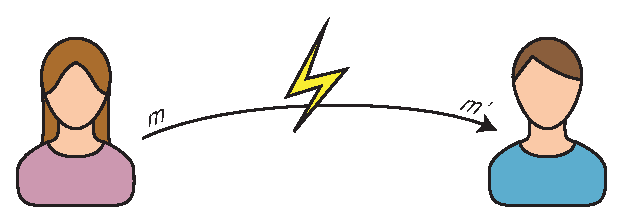
\includegraphics[width=10cm]{img/usage1.eps}
    \caption{Wiadomość odebrana przez Boba niekoniecznie musi dotrzeć do niego
    w~formie identycznej jak podczas nadania przez Alicję}
    \label{fig:usage_integrity_check_1}
\end{figure}

Z~taką transmisją wiąże się wiele problemów, gdy zaczniemy rozpatrywać ją pod
kątem zapewnienia bezpieczeństwa. Jednym z~takim problemów jest zapewnienie
bezpiecznego mechanizmu weryfikacji, czy dane odebrane przez Boba są faktycznie
tymi samymi danymi, które były wysłane do niego przez Alicję, a~więc czy nie
zostały zmienione w~jakikolwiek sposób podczas transportu. Innymi słowy, należy
w~jakiś sposób zweryfikować, czy $m' = m$.

Z~pomocą w~rozwiązaniu tego problemu przychodzą funkcje haszujące. Alicja może,
obok samej wiadomości $m$, przesłać wyliczony u~siebie skrót tej wiadomości,
$h=H(m)$. Bob może wówczas zweryfikować integralność odebranych danych $m'$
poprzez obliczenie ich skrótu po swojej stronie $H(m')=h'$, a~w~następnej
kolejności porównanie samych skrótów (sprawdzenie, czy obliczony przez Alicję
$h$ jest równy obliczonemu przez niego $h'$).

\begin{figure}[htb!]
    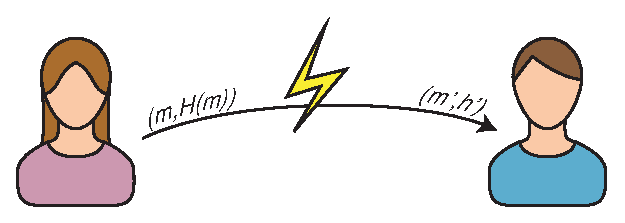
\includegraphics[width=10cm]{img/usage1b.eps}
    \caption{Bob ma teraz dodatkowy mechanizm weryfikacji integralności~--
    wystarczy, że sprawdzi, czy $H(m')=h'$.}
    \label{fig:usage_integrity_check_2}
\end{figure}

Wprowadzenie funkcji haszujących właśnie pozwoliło sprowadzić problem
zabezpieczenia transmisji potencjalnie bardzo długich komunikatów do
zabezpieczenia transmisji jedynie samych skrótów.

Należy zdawać sobie sprawę, że nie rozwiązuje to problemu zabezpieczenia
transmisji przed rozmyślnymi atakami~-- jeśli ktoś mógł wcześniej zmieniać
zawartość $m$, teraz może również zmienić wartość $h$ zawierającą $H(m)$.
Ponadto funkcje haszujące nie zapewniają żadnej poufności danych. Mimo to z~ich
zastosowania płyną pewne wymienione niżej korzyści.

\begin{itemize}

    \item Rozwiązanie to jest przydatne w~sytuacjach, kiedy nie mamy do
    czynienia z~rozmyślnymi atakami, a~jedynie przypadkowymi zakłóceniami~--
    prawdopodobieństwo, że skrót $H(m')$ będzie równy $H(m)$ w~sytuacji, kiedy
    $m \neq m'$ będzie minimalne. Jest to jedno z~naturalnych zastosowań
    funkcji haszujących, w~których odgrywają rolę trudnej do podrobienia sumy
    kontrolnej.

    \item Ponadto ułatwione jest tworzenie innych protokołów~-- dzięki funkcjom
    haszującym zależy nam na zabezpieczeniu przed modyfikacją nie całej
    wiadomości, a~jedynie jej malutkiego kawałka zawierającego skrót.
    Przykładem protokołu, który pracuje na opisanej powyżej zasadzie, jest
    podpis elektroniczny~-- \latin{de~facto} weryfikuje się tam wyłącznie
    autentyczność skrótu wiadomości, a~nie samą wiadomość.

\end{itemize}



\subsubsection{Bezpieczne przechowywanie / weryfikacja haseł}
\label{sec:usage_password_check}
Funkcje haszujące przychodzą z~pomocą także w~technikach przechowywania haseł.
Wyobraźmy sobie przeciętny mechanizm autentykacji.

\begin{myenumerate}

    \item Użytkownik Alicja przesyła swoje dane uwierzytelniające do serwera.

    \item Serwer odbiera dane $m$.

    \item Serwer porównuje dane $m$ z~wzorcem $m'$ przechowywanym w~bazie
    danych: \label{enu:server_pass_check}

    \begin{myenumerate}

        \item jeżeli dane się zgadzają ($m = m'$), serwer udziela Alicji
        dostępu,

        \item w~przeciwnym wypadku odmawia dostępu.

    \end{myenumerate}

\end{myenumerate}

Z~takim podejściem wiążą się pewne problemy. Po pierwsze, dane, która przesyła
Alicja, mogą zostać przechwycone przez osobę trzecią, zatem wymagają
zaszyfrowania (np. poprzez zaszyfrowanie transmisji protokołem \texttt{HTTPS}).
Jednak nie ten problem okazuje się ważny z~punktu widzenia funkcji haszujących.
Nas zainteresuje problem wiążący się z~punktem~\ref{enu:server_pass_check}~--
co w~wypadku, kiedy do bazy danych serwera, z~jakichkolwiek przyczyn, uzyskuje
dostęp ktoś niepożądany? Taka osoba może wówczas podejrzeć dane
uwierzytelniające \emph{wszystkich} użytkowników, także Alicji, a~następnie
pomyślnie zalogować się przy pomocy tak wykradzionych danych.

Musimy zatem jakoś zabezpieczyć bazę danych. Można próbować ją szyfrować lub
inaczej zabezpieczać dane w~niej przechowywane, problem z~takim podejściem jest
jednak taki, że na pewnym poziomie tak czy inaczej jakaś osoba (administrator)
zawsze będzie miał dostęp do fizycznych danych. Możemy także zahaszować dane
uwierzytelniające i~zmodyfikować nasz protokół w~sposób opisany poniżej.

\label{sec:secure_pasword_storage}
\begin{myenumerate}

    \item Użytkownik Alicja przesyła swoje dane uwierzytelniające do serwera.

    \item Serwer odbiera dane $m$.

    \item Serwer wylicza na ich podstawie hasz $h = H(m)$.

    \item Serwer porównuje hasz $h$ z~wzorcowym haszem $h'$ przechowywanym
    w~bazie danych:

    \begin{myenumerate}

        \item jeżeli skróty się zgadzają ($h = h'$), serwer udziela Alicji
        dostępu,

        \item w~przeciwnym wypadku odmawia dostępu.

    \end{myenumerate}

\end{myenumerate}

Dzięki temu, że w~bazie przechowywane są jedynie nieodwracalne skróty, nawet
w~przypadku kradzieży bazy danych na podstawie wykradzionych skrótów nie
powinno być można odtworzyć oryginalnych danych (patrz
punkt~\ref{sec:preimage_resistance}). Teoretycznie zatem atakującemu taka baza
w~zasadzie do niczego się nie przyda.

Należy jednak zwrócić uwagę, że protokół ten nie jest bezpieczny bez pewnych
poprawek. Przyczyny i~natura poprawek omówione są
w~części~\ref{sec:universal_attacks}.



\subsubsection{Jednoznaczna identyfikacja danych}
Innym zastosowaniem funkcji haszujących jest identyfikacja ciągów bajtów,
a~w~szerszym ujęciu~-- plików, struktur/obiektów programistycznych itp. Poniżej
znajdują się przykłady wykorzystania tego pomysłu w~różnego rodzaju
rozwiązaniach.

\begin{itemize}

    \item Systemy kontroli wersji, w~tym Mercurial oraz Git, wykorzystują
    funkcje skrótu w~celu bezpiecznej identyfikacji konkretnych wersji pliku,
    numerowania kolejnych zmian i~bezpiecznego przechowywania historycznej
    struktury repozytorium.

    \item Linki ed2k oraz magnet, używane w~sieciach peer-to-peer, wykorzystują
    funkcje skrótu w~celu lokalizacji źródeł, skąd dany plik może być pobrany,
    a~także weryfikacji już ściągniętych danych (patrz
    punkt~\ref{sec:usage_integrity_check}).

    \item Struktury danych takie jak tablice mieszające (tzn. tablice, których
    kluczami może być dowolny obiekt, w~przeciwieństwie do klasycznych tablic
    o~indeksach liczbowych), wykorzystują funkcje haszujące do serializacji
    dowolnych obiektów na taką postać, jaką ich algorytmy indeksowania są
    w~stanie obsłużyć. Przykładowo, w~języku Java każdy zdefiniowany przez
    użytkownika obiekt powinien zaimplementować metodę \texttt{hashCode()},
    która w~zamierzeniu ma pozwolić łatwo odróżniać (na~tyle, na~ile to
    możliwe) konkretne instancje obiektu w~stosunku do pozostałych.

\end{itemize}

\begin{figure}[bht]
    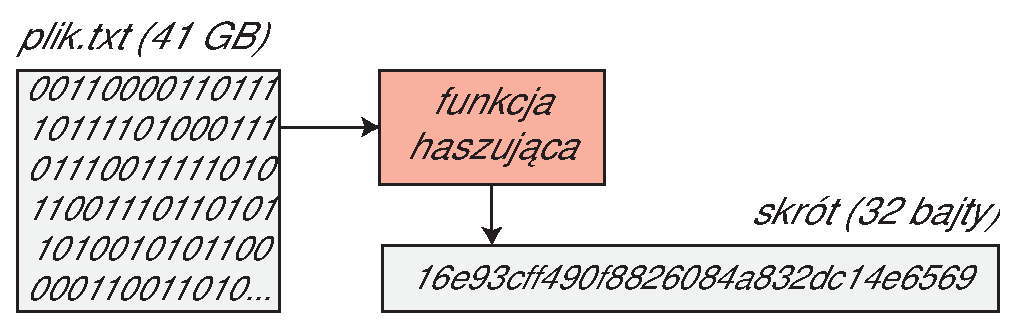
\includegraphics[width=12cm]{img/usage3.eps}
    \caption{Gdy trzeba zweryfikować poprawność przesłania dużej struktury,
    łatwiej porównać krótki skrót}
\end{figure}

Biorąc pod uwagę fakt, że kryptograficzne funkcje skrótu są dużo bardziej
kosztowne obliczeniowo niż zwykłe, nieodporne na ataki funkcje haszujące,
w~większości tego typu zastosowań korzystanie z~kryptograficznych funkcje
skrótu postrzegane jest jako przesada i~stosowane są zwyczajne funkcje skrótu.
Mimo to, czasem jednak bezpieczeństwo jest konieczne, szczególnie w~sytuacjach
opisanych powyżej, gdzie ryzyko ataku jest wysokie. Przykładowo, atakujący może
stworzyć plik zawierający wirus, którego hasz byłby taki sam jak skrót całkiem
niewinnego pliku, po czym umieścić taki plik w~sieci peer-to-peer~-- dzięki
zastosowaniu kryptograficznych funkcji skrótu, taki scenariusz jest bez
porównania trudniejszy do skutecznego przeprowadzenia.



\subsection{Rys historyczny}
Historia funkcji haszujących sięga późnych lat 70--tych. W~roku 1976 Diffie
i~Hellman w~swojej pracy traktującej o~kryptografii z~kluczem publicznym,
opisali zapotrzebowanie na funkcję mapującą ciągi bitów dowolnej długości na
ciągi bitów ograniczonej długości w~nieodwracalny sposób. W~roku 1978 Rabin po
raz pierwszy zaproponował funkcję skrótu opartą na 64--bitowym wariancie
blokowego algorytmu szyfrującego DES. W~1979 roku Yuval opisał sposób, jak
wykorzystując paradoks urodzinowy złamać $n$--bitową funkcję haszującą w~czasie
$2^{n/2}$.

W~tym samym roku zaczęły się pojawiać pierwsze próby zdefiniowania warunków,
jakie powinny spełniać bezpieczne funkcje skrótu. W~1979 Merkle wprowadził
pojęcie odporności na kolizje oraz odporności pierwszego i~drugiego rzędu
(patrz sekcja~\ref{sec:secure_hash_attributes}). Definicje te zostały
ostatecznie sformalizowane przez Damg\r{a}rda w~roku 1987. W~roku 2004 Rogaway
i~Shrimpton pokazali, że funkcje haszujące w~miarę możliwości nie powinny być
odróżnialne od \en{random oracles}.

Już od samego początku, czyli późnych lat 70--tych, funkcje haszujące
przeżywały bardzo szybki rozwój. Zapotrzebowanie na bezpieczne i~szybkie
funkcje skrótu było szeroko rozumiane, nie zaskakuje zatem fakt, że do lat
90--tych znane było już około 50 konstrukcji. Pierwsi kandydaci korzystali
z~dorobku blokowych funkcji szyfrujących; w~późniejszym okresie rozwoju
niektórzy poszli w~kierunku teoretycznych konstrukcji opartych na algebrze
liniowej. Z~czasem jednak zaniechano adaptowania mechanizmów sprawdzonych
w~innych zastosowaniach na rzecz tworzenia dedykowanych funkcji.

Tak naprawdę do dnia dzisiejszego niewiele się zmieniło: od lat mamy do
czynienia z~ciągłym procesem wykazywania słabości istniejących rozwiązań
i~w~odpowiedzi wymyślania kolejnych usprawnień bądź całkiem nowych konstrukcji.
Proces ten zyskał nawet niedawno własne wydarzenie medialne w~postaci konkursu
ogłoszonego przez \enn{National Institute of Standards and Technology}, mającego
na celu wyłonienie następcy funkcji haszujących \texttt{SHA-1} i~\texttt{SHA-2}
spośród kilkudziesięciu kandydatów zgłoszonych przez kryptologów z~całego
świata. Cykl ten będzie prawdopodobnie trwał tak długo, aż zostanie odkryta
uniwersalna nieodwracalna funkcja skrótu lub wykazana zostanie niemożność
stworzenia takowej.
